%%%%%%%%%%%%%%%%%%%%%%%%%%%%%%%%%%%%%%%%%%%%%%%%%%%%%%%%%%%%%%%%%%%%%%%%%%%%%%
%%% 				Customizações do abnTeX2 para o IFCE    			   %%%
%%% 		Instituto Federal de Educação, Ciência e Tecnologia do Ceará   %%%
%%%																	       %%%
%%% Template disponível em: https://github.com/clodomirneto/IFCETeX2	   %%%
%%% Desenvolvedores do IFCETeX2: Professor Clodomir Silva Lima Neto	       %%%
%%% 							 Professor Marcelo Araújo Lima		       %%%
%%% 					  	     Professor Antonio Sergio de Sousa Vieira  %%%
%%% E-mails para contato: clodomir.neto@ifce.edu.br						   %%%
%%% 					  marcelo.alima@ifce.edu.br					       %%%
%%% 					  sergio.vieira@ifce.edu.br					       %%%
%%%																		   %%%
%%% Agradecimento: Thiago Nascimento 									   %%%
%%% https://github.com/thiagodnf/uecetex2                                  %%%
%%%%%%%%%%%%%%%%%%%%%%%%%%%%%%%%%%%%%%%%%%%%%%%%%%%%%%%%%%%%%%%%%%%%%%%%%%%%%%

%%%%%%%%%%%%%%%%%%%%%%%%%%%%%%%%%%%%%%%%%%%%%%%%%%%%%%%%%%%%%%%%%%%%%%%%%%%%%%
%%% 			Instruções para Uso do Template IFCETeX2	  			   %%%
%%%																	       %%%
%%% 1. Criar uma conta no Overleaf.									       %%%
%%% 2. No Ambiente Overleaf, clicar em Menu (canto superior esquerdo) 	   %%% 
%%% 3. Clicar em "Copiar Projeto".  									   %%%
%%% 4. Dê um novo nome para o Projeto. 								       %%%
%%%%%%%%%%%%%%%%%%%%%%%%%%%%%%%%%%%%%%%%%%%%%%%%%%%%%%%%%%%%%%%%%%%%%%%%%%%%%%

%%%%%%%%%%%%%%%%%%%%%%%%%%%%%%%%%%%%%%%%%%%%%%%%%%%%%%%%%%%%%%%%%%%%%%%%%%
%%% Customizações do abnTeX2 para o Campus Crateús do IFCE    			%%%
%%% Instituto Federal de Educação, Ciência e Tecnologia do Ceará.   	%%%
%%%																	%%%
%%% Template disponível em: https://github.com/clodomirneto/IFCETeX2	%%%
%%% Desenvolvedor do IFCETeX2: Professor Clodomir Silva Lima Neto  	%%%
%%% Email para contato: clodomir.neto@ifce.edu.br						%%%
%%% 																	%%%
%%% Agradecimento: Thiago Nascimento 									%%%
%%% https://github.com/thiagodnf/uecetex2                              %%%
%%%%%%%%%%%%%%%%%%%%%%%%%%%%%%%%%%%%%%%%%%%%%%%%%%%%%%%%%%%%%%%%%%%%%%%%%%

%%%%%%%%%%%%%%%%%%%%%%%%%%%%%%%%%%%%%%%%%%%%%%%%%%%%%%%%%%%%%%%%%%%%%%%%%%
%%% 						Sequência do GitHub							%%%
%%%																	%%%
%%% git status + git add . + git commit + git push					%%%
%%%%%%%%%%%%%%%%%%%%%%%%%%%%%%%%%%%%%%%%%%%%%%%%%%%%%%%%%%%%%%%%%%%%%%%%%%

\documentclass[        
    a4paper,          % Tamanho da folha A4
    12pt,             % Tamanho da fonte 12pt
    chapter=TITLE,    % Todos os capitulos devem ter caixa alta
    %section=TITLE,    % Todas as secoes devem ter caixa alta
    oneside,          % Usada para impressao em apenas uma face do papel
    english,          % Hifenizacoes em ingles
    spanish,          % Hifenizacoes em espanhol
    brazil            % Ultimo idioma eh o idioma padrao do documento
]{abntex2}

% Importações de pacotes
\usepackage[utf8]{inputenc}                         % Acentuação direta
\usepackage[T1]{fontenc}                            % Codificação da fonte em 8 bits
\usepackage{graphicx}                               % Inserir figuras
\usepackage{amsfonts,amssymb,amsmath}             % Fonte e símbolos matemáticos
\usepackage{booktabs}                               % Comandos para tabelas
\usepackage{verbatim}                               % Texto é interpretado como escrito no documento
\usepackage{multirow,array}                        % Múltiplas linhas e colunas em tabelas
\usepackage{indentfirst}                            % Endenta o primeiro parágrafo de cada seção.
\usepackage{listings}                               % Utilizar codigo fonte no documento
\usepackage{xcolor}
\usepackage{microtype}                              % Para melhorias de justificação?
\usepackage[portuguese,ruled,lined]{algorithm2e}    % Escrever algoritmos
\usepackage{algorithmic}                            % Criar Algoritmos  
%\usepackage{float}                                  % Utilizado para criação de floats
\usepackage{amsgen}
\usepackage{lipsum}                                 % Usar a simulação de texto Lorem Ipsum
%\usepackage{titlesec}                               % Permite alterar os títulos do documento
\usepackage{tocloft}                                % Permite alterar a formatação do Sumário
\usepackage{etoolbox}                               % Usado para alterar a fonte da Section no Sumário
\usepackage[nogroupskip,nonumberlist,acronym]{glossaries}                % Permite fazer o glossario
\usepackage{caption}                                % Altera o comportamento da tag caption
\usepackage[alf,abnt-emphasize=bf,bibjustif, recuo=0cm,abnt-etal-cite=3,abnt-etal-list=0,abnt-etal-text=it]{abntex2cite}  % Citações padrão ABNT
%\usepackage[bottom]{footmisc}                      % Mantém as notas de rodapé sempre na mesma posição
%\usepackage{times}                                 % Usa a fonte Times
\usepackage{mathptmx}                               % Usa a fonte Times New Roman							
%\usepackage{lmodern}                               % Usa a fonte Latin Modern
%\usepackage{subfig}                                % Posicionamento de figuras
%\usepackage{scalefnt}                              % Permite redimensionar tamanho da fonte
%\usepackage{color, colortbl}                       % Comandos de cores
%\usepackage{lscape}                                % Permite páginas em modo "paisagem"
%\usepackage{ae, aecompl}                           % Fontes de alta qualidade
%\usepackage{picinpar}                              % Dispor imagens em parágrafos
%\usepackage{latexsym}                              % Símbolos matemáticos
%\usepackage{upgreek}                               % Fonte letras gregas
\usepackage{appendix}                               % Gerar o apendice no final do documento
\usepackage{paracol}                                % Criar paragrafos sem identacao
\usepackage{ifcetex2}		                        	  % Biblioteca com as normas do IFCE para trabalhos academicos
\usepackage{pdfpages}                               % Incluir pdf no documento
\usepackage{textcomp}
% Organiza e gera a lista de abreviaturas, simbolos e glossario
\makeglossaries
% Gera o Indice do documento
\makeindex

%TEOREMAS

\newtheorem{proposition}{Proposição}[chapter]
\newtheorem{theorem}{Teorema}[chapter]
\newtheorem{lemma}{Lema}[chapter]
\newtheorem{definition}{Definição}[chapter]
\newtheorem{exemplo}{Exemplo}[chapter]
\newtheorem{corollary}{Corolário}[chapter]
\newtheorem{exercicio}{Exercício}[chapter]

%PROVAS

\newenvironment{prova}[1][Prova]{\noindent\textbf{#1.} }{\hfill\rule{0.5em}{0.5em}}
\newenvironment{exm}{\noindent{\textbf{Exemplo:}}}{$\diamond$}
\newenvironment{dem}[1][Demonstra\c c\~ao]{\noindent\textbf{#1.} }{\hfill\rule{2mm}{2mm}}

% Opções disponíveis

%\trabalhoacademico{tese}
%\trabalhoacademico{dissertacao}
%\trabalhoacademico{tccespecializacao}
\trabalhoacademico{tccgraduacao}

% Define se o trabalho é uma qualificação, coloque 'nao' para versão final do trabalho

\ehqualificacao{nao}

% Remove as bordas vermelhas e verdes do PDF gerado, coloque 'sim' para remover

\removerbordasdohyperlink{sim} 

% Adiciona a cor azul a todos os hyperlinks

\cordohyperlink{nao}

% Informação relacionadas ao trabalho

\autor{Nome Completo do Autor}
\titulo{Título do Trabalho: Subtítulo (se houver)}
\local{Cidade - UF}
\data{Ano de Entrega}

% Informação sobre a IES

\ies{Instituto Federal de Educação, Ciência e Tecnologia do Ceará}
\iessigla{IFCE}
\centro{\textit{Campus} Crateús}

% Informação para Tese

\programadoutorado{Programa de Pós-Graduação em Saúde Coletiva}
\nomedodoutorado{Doutorado em Saúde Coletiva}
\doutorem{Saúde Coletiva}
\areadeconcentracaodoutorado{Saúde Coletiva}

% Informação para Dissertacao

\programamestrado{Programa de Pós-Graduação em Ciência da Computação}
\nomedomestrado{Mestrado Acadêmico em Ciência da Computação}
\mestreem{Ciência da Computação}
\areadeconcentracaomestrado{Ciência da Computação}

% Informação para TCC de Especialização

\especializacaoem{Ensino de Ciências da Natureza e Matemática}
\habilitacaoesp{Especialista}
\areadeconcentracaoespecializacao{Ensino de Matemática}

% Informação para TCC de Graduação

\graduacaoem{Licenciatura em Matemática} 
\habilitacao{Licenciado} % Licenciado ou Bacharel
\areadeconcentracaograduacao{Matemática}

% Data de Aprovação

\dataaprovacao{\underline{\hspace*{1cm}}/\underline{\hspace*{1cm}}/\underline{\hspace*{1.2cm}}.}

% Abreviaturas dos títulos acadêmicos

% Especialista: Esp.
% Mestre: Me.
% Mestra: Ma.
% Doutor: Dr.
% Doutora: Dra.

% Informação sobre o Orientador

\orientador{Prof. Dr. XXXXX}
\orientadories{Instituto Federal de Educação, Ciência e Tecnologia do Ceará}
\orientadoriessigla{IFCE}
\orientadorcentro{\textit{Campus} Crateús}
\orientadorfeminino{nao} % Coloque 'sim' se for do sexo feminino

% Informação sobre o Coorientador

\coorientador{Profa. Ma. XXXXX} % Deixe o nome do coorientador em branco para remover do documento
\coorientadories{Instituto Federal de Educação, Ciência e Tecnologia do Ceará}
\coorientadoriessigla{IFCE}
\coorientadorcentro{\textit{Campus} Crateús}
\coorientadorfeminino{sim} % Coloque 'sim' se for do sexo feminino

% Informação sobre a banca

% Membro da Banca Dois

\membrodabancadois{Prof. Dra. XXXXX}
\membrodabancadoisies{Instituto Federal de Educação, Ciência e Tecnologia do Ceará}
\membrodabancadoisiessigla{IFCE}
\membrodabancadoiscentro{\textit{Campus} Crateús}

% Membro da Banca Três

\membrodabancatres{Prof. Dra. XXXXX}
\membrodabancatresies{Instituto Federal de Educação, Ciência e Tecnologia do Ceará}
\membrodabancatresiessigla{IFCE}
\membrodabancatrescentro{\textit{Campus} Crateús}

% Informação Complementar sobre a banca

\membrodabancaquatro{Membro da Banca Quatro}
\membrodabancaquatrocentro{Centro de Ciências e Tecnologia - CCT}
\membrodabancaquatroies{Universidade do Membro da Banca Quatro - SIGLA}
\membrodabancacinco{Membro da Banca Cinco}
\membrodabancacincocentro{Teste}
\membrodabancacincoies{Universidade do Membro da Banca Cinco - SIGLA}
\membrodabancaseis{Membro da Banca Seis}
\membrodabancaseiscentro{}
\membrodabancaseisies{Universidade do Membro da Banca Seis - SIGLA}

\begin{document}	

% Elementos pré-textuais

\imprimircapa
\imprimirfolhaderosto{}
\imprimirfichacatalografica{elementos-pre-textuais/ficha-catalografica}
%\imprimirerrata{elementos-pre-textuais/errata}
\imprimirfolhadeaprovacao
\imprimirdedicatoria{elementos-pre-textuais/dedicatoria}
\imprimiragradecimentos{elementos-pre-textuais/agradecimentos}
\imprimirepigrafe{elementos-pre-textuais/epigrafe}
\imprimirresumo{elementos-pre-textuais/resumo}
\imprimirabstract{elementos-pre-textuais/abstract}
\imprimirlistadefiguras
\imprimirlistadetabelas
%\imprimirlistadequadros
%\imprimirlistadealgoritmos
%\imprimirlistadecodigosfonte
\imprimirlistadesiglas{elementos-pre-textuais/lista-de-siglas}
\imprimirlistadesimbolos{elementos-pre-textuais/lista-de-simbolos}
\imprimirsumario
	
% Elementos textuais

\textual
\chapter{Introdução}

Tem como finalidade explicar para o leitor do que trata a pesquisa, apresentando, de maneira sucinta, o tema do trabalho e sua delimitação, a problematização, os objetivos, a justificativa, as hipóteses e variáveis (\cite{andrade}; \cite{koche}; \cite{medeiros}).

Pode-se, também, indicar os principais teóricos que fundamentaram a pesquisa e descrever brevemente os assuntos abordados nas demais seções do trabalho \cite{medeiros}.

O texto deve ser justificado, digitado em fonte \textit{Times New Roman} ou Arial, tamanho 12 e espaçamento de 1,5 entre as linhas, com exceção das citações com mais de três linhas, notas de rodapé e paginação, que devem ser em fonte tamanho 10 e espaçamento simples (1,0).
\chapter{Título da Seção Primária do Desenvolvimento}

\begin{SingleSpace}
\begin{flushright}
\begin{minipage}[b]{8cm}
\begin{small}
``Podem, também, constar epígrafes nas folhas ou páginas de abertura das seções primárias (capítulos)'' (AUTOR, ano, página).
\end{small}
\end{minipage}
\end{flushright}
\end{SingleSpace}

Após o capítulo introdutório, iniciam-se os capítulos do desenvolvimento do estudo. É a parte principal do trabalho, na qual se apresentam a revisão de literatura, os procedimentos metodológicos adotados, a exposição, análise e interpretação dos dados \cite{koche,marconi}.

Divide-se, sistematicamente, em seções e subseções, da primária à quinária, derivadas do tema geral do trabalho \cite{barros}. Todas as seções e subseções devem conter um texto relacionado a elas.

Todo texto deve ser justificado, digitado em fonte \textit{Times New Roman} ou Arial, tamanho 12 e espaçamento de 1,5 entre as linhas, com exceção das citações com mais de três linhas, notas de rodapé, paginação, legendas e fontes das ilustrações e das tabelas, que devem ser em fonte tamanho 10 e espaçamento simples (1,0).

\section{Título da Seção Secundária}

No Brasil, a criação de uma organização nacional de normalização estava voltada ao mercado da construção civil. Em 1940, foi consolidada a Associação Brasileira de Normas Técnicas (ABNT), reconhecida posteriormente, em 1979, como o único Foro Nacional de Normalização.

A ABNT define norma técnica como:

\begin{SingleSpace}
\begin{flushright}
\begin{minipage}[b]{12cm}
\begin{small}
Documento, estabelecido por consenso e aprovado por um organismo reconhecido, que fornece, para um uso comum e repetitivo, regras, diretrizes ou características para atividades ou seus resultados, visando à obtenção de um grau ótimo de ordenação em um dado contexto (ASSOCIAÇÃO BRASILEIRA DE NORMAS TÉCNICAS, 2006, p. 4, grifo do autor).
\end{small}
\end{minipage}
\end{flushright}
\end{SingleSpace}

O uso das normas se tornou um diferencial competitivo para grandes empresas e aos poucos se consolidava a criação de um mercado nacional. A necessidade desses padrões formais é defendida por \citeonline[p. 62]{cunha}:

\begin{SingleSpace}
\begin{flushright}
\begin{minipage}[b]{12cm}
\begin{small}
Todo trabalhador intelectual precisa aceitar a responsabilidade de comunicar adequada e amplamente os resultados de seus estudos e pesquisas, adotando, para tanto, a mesma seriedade, dedicação e disposição de espírito com que encara a responsabilidade de planejar e executar os estudos e as pesquisas que lhe cabem.
\end{small}
\end{minipage}
\end{flushright}
\end{SingleSpace}

Etimologicamente, a palavra conhecimento vem do latim cognoscere e quer dizer vir a saber. Em outras palavras, ``[…] é a relação que se estabelece entre o sujeito que conhece e o objeto que é conhecido'' \cite[p. 5]{cervo}.

Como afirma \citeonline[p. 24]{witter}, ``[…] a sala de aula é um laboratório de pesquisa […]''.

\subsection{Título da seção terciária}

Todas as seções e subseções devem conter um texto relacionado a elas.

\subsubsection{Título da seção quaternária}

As ilustrações - desenhos, esquemas, fluxogramas, fotografias, gráficos, mapas, organogramas, plantas, quadros, retratos, figuras, imagens, entre outros - devem ser inseridas o mais próximo possível do texto a que se referem.

Sua identificação aparece na parte superior, composta pelo nome específico da ilustração, seguido do número de ordem de ocorrência no texto, em algarismos arábicos, travessão e do respectivo título, ajustados às margens da ilustração, em espaço simples (1,0) e alinhamento justificado.

Na Figura 1, apresenta-se a distribuição dos Campi do IFCE pelo estado cearense.

\begin{figure}[!ht]
\Caption{Distribuição dos campi do Instituto Federal de Educação, Ciência e Tecnologia do Ceará}
\centering
\label{fig:exemplo-1}
\IFCEfig{}{
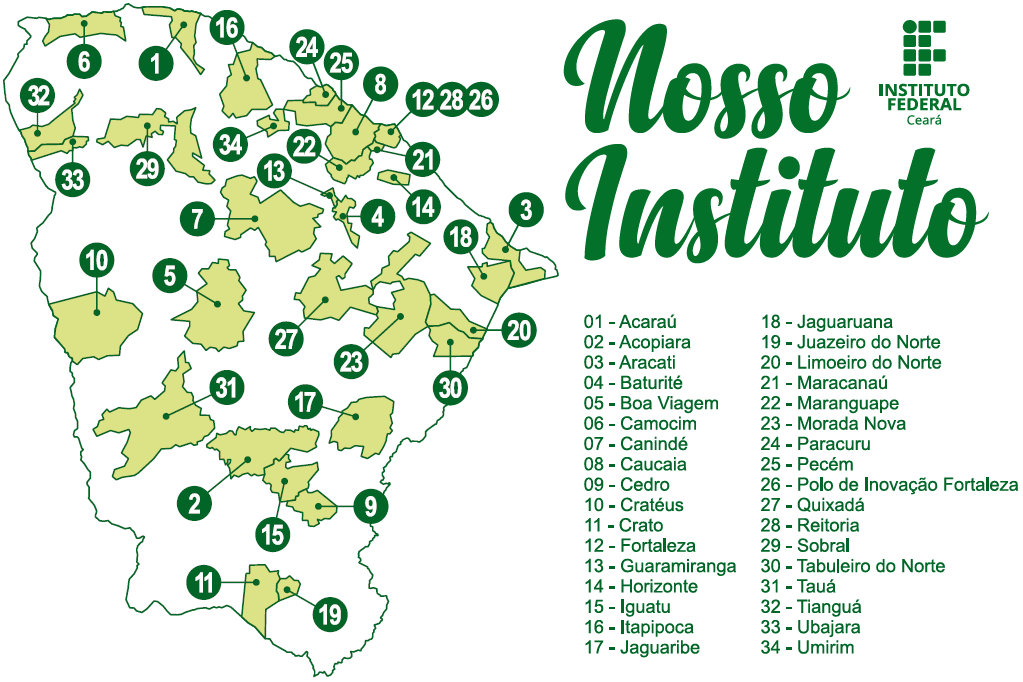
\includegraphics[scale=0.5]{figuras/ifce-estado}
}{
\Fonte{Instituto Federal de Educação, Ciência e Tecnologia do Ceará (2018).}
}
\end{figure}

\newpage

\subsubsubsection{Título da seção quinária}

As tabelas - apresentação de informações, de forma não discursiva, nas quais o dado numérico se destaca como informação central - devem ser inseridas o mais próximo possível do texto a que se referem.

Sua identificação aparece na parte superior, composta pelo nome tabela, seguido do número de ordem de ocorrência no texto, em algarismos arábicos, travessão e do respectivo título, ajustados às margens da tabela, em espaço simples (1,0) e alinhamento justificado.

\begin{table}[!ht]	
\Caption{Estimativas populacionais brasileiras - Regiões - 2011-2017}
\centering
\label{tab:exemplo-1}		
\IFCEtab{}{
\begin{tabular}{c|c|c|c|c|c}
\hline
& \multicolumn{5}{c}{\textbf{Regiões}} \\
\cline{2-6}
\textbf{Ano} & \textbf{Sudeste} & \textbf{Nordeste} & \textbf{Sul} & \textbf{Norte} & \textbf{Centro-Oeste} \\
\hline
2011 & 80.975.616 & 53.501.859 & 27.562.433 & 16.095.187 & 14.244.192 \\
\hline
2012 & 81.565.983 & 53.907.144 & 27.708.514 & 16.303.145 &
14.419.229 \\
\hline
2013 & 84.465.570 & 55.794.707 & 28.795.762 & 16.983.484 &
14.993.191 \\
\hline
2014 & 85.115.623 & 56.186.190 & 29.016.114 & 17.231.027 &
15.219.608 \\
\hline
2015 & 85.745.520 & 56.559.481 & 29.230.180 & 17.472.636 &
15.442.232 \\
\hline
2016 & 86.356.952 & 56.915.936 & 29.439.773 & 17.707.783 &
15.660.988 \\
\hline
2017 & 86.949.714 & 57.254.159 & 29.644.948 & 17.936.201 &
15.875.907 \\
\hline
\end{tabular}
}{
\Fonte{Instituto Brasileiro de Geografia e Estatística (2018).}
\vspace*{-0.6cm}
\begin{flushright}
\begin{minipage}[b]{13.9cm}
\begin{SingleSpace}
\begin{footnotesize}
Notas: Em 2012: \\
\hspace*{0.9cm}
1 - Por determinação judicial e para efeito de distribuição do Fundo de Participação dos Municípios, a população do Município de Brasil Novo-PA é de 17.960 habitantes. Processo Judicial nº 1-28.2012.4.01.3903. \\
\hspace*{0.9cm} 2 - Por determinação judicial e para efeito de distribuição do Fundo de Participação dos Municípios, a população do Município de Jacareacanga-PA é de 41.487 habitantes. Processo Judicial nº 798-41.2011.4.01.3902, Seção Judiciária de Itaituba-PA. \\
\hspace*{0.9cm} Em 2013: \\
\hspace*{0.9cm} Por determinação judicial e para efeito de distribuição do Fundo de Participação dos Municípios, a população do Município de Jacareacanga-PA é de 41.487 habitantes. Processo Judicial nº 798-41.2011 4.01.3902 Seção Judiciária de Itaituba-PA. \\
\hspace*{0.9cm} Em 2014: \\
\hspace*{0.9cm}1 - Por determinação judicial e para efeito de distribuição do Fundo de Participação dos Municípios, a população do Município de Jacareacanga-PA é de 41.487 habitantes. Processo Judicial nº 798-41.2011.4.01.3902, Seção Judiciária de Itaituba-PA. \\
\hspace*{0.9cm} 2 - Por determinação judicial o Município de Coronel João Sá - BA teve os efeitos das estimativas das populações de 2014, 2015 e 2016 suspensas, passando a vigorar, para efeito de distribuição do Fundo de Participação dos Municípios, a população estimada para o ano de 2013, que foi de 17.422 habitantes. Processo Judicial nº 0002222-53.2017.4.01.3306 - Vara Única de Paulo Afonso-BA.
\end{footnotesize}
\end{SingleSpace}
\end{minipage}
\end{flushright}
}
\end{table}

\newpage

Além do número da população residente, foram extraídas do Portal do IBGE informações populacionais com as variáveis apresentadas no quadro a seguir.

A identificação do quadro aparece na parte superior, composta por seu nome, seguido do número de ordem de ocorrência no texto, em algarismos arábicos, travessão e do respectivo título, ajustados às margens do quadro, em espaço simples (1,0) e alinhamento justificado\footnote{As notas de rodapé têm por finalidade prestar esclarecimentos ou fazer considerações sobre certos aspectos que não devem ser incluídos no texto para não interromper a sequência lógica da leitura.}.

\begin{quadro}[!ht]	
\Caption{Características da população brasileira pesquisadas}
\centering
\label{qua:exemplo-1}
\IFCEqua{}{
\begin{tabular}{|l|l|}
\hline
\textbf{Tema} & \textbf{Variáveis} \\
\hline
Características gerais da população & População residente, situação de domicílio, sexo e idade \\
\hline
Cor ou raça & População residente, idade, sexo, situação de domicílio, educação \\
\hline
Educação & Taxa de alfabetização \\
\hline
Emigração & Emigrantes internacionais \\
\hline
Registro de nascimento & Idade, situação de domicílio, sexo, cor ou raça \\
\hline
Trabalho e rendimento & Idade, sexo, cor ou raça, Índice de Gini \\
\hline
\end{tabular}
}{
\Fonte{Instituto Brasileiro de Geografia e Estatística (2010).}
}
\end{quadro}

\newpage

Para acompanhar o crescimento populacional\footnote{As notas devem constar na mesma página em que ocorre a chamada numérica no texto, digitadas com espaçamento simples (1,0) entre as linhas e alinhadas, a partir da segunda linha da mesma nota, abaixo da primeira letra da primeira palavra, de forma a destacar o expoente, sem espaço entre elas e com fonte tamanho 10.}, anualmente, o IBGE publica estimativas populacionais do nosso país, com dados das regiões, dos estados e, até, dos 5.570 municípios brasileiros\footnote{As notas podem ser de dois tipos: notas de referência e notas explicativas, conforme o Manual de Normalização de Trabalhos Acadêmicos do IFCE.}. 
%\chapter{Trabalhos Relacionados}
\label{cap:trabalhos-relacionados}

Integer non lacinia magna. Aenean tempor lorem tellus, non sodales nisl commodo ut. Proin mattis placerat risus sit amet laoreet. Praesent sapien arcu, maximus ac fringilla efficitur, vulputate faucibus sem. Donec aliquet velit eros, sit amet elementum dolor pharetra eget. Integer eget mattis libero

\section{Trabalho Relacionado A}
\label{sec:trabalho-relacionado-a}

\lipsum[10]

	\begin{figure}[h!]
		\centering
		\Caption{\label{fig:exemplo-1} Lorem ipsum dolor sit amet, consectetur adipiscing elit. Suspendisse commodo lectus et augue elementum varius.}	
		\IFCEfig{}{
			\fbox{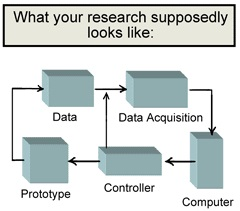
\includegraphics[width=8cm]{figuras/figura-1}}
		}{
			\Fonte{Elaborado pelo autor}
		}	
	\end{figure}
	
\lipsum[11]

\section{Trabalho Relacionado B}
\label{sec:trabalho-relacionado-b}

Integer non lacinia magna. Aenean tempor lorem tellus, non sodales nisl commodo ut. Proin mattis placerat risus sit amet laoreet. Praesent sapien arcu, maximus ac fringilla efficitur, vulputate faucibus sem. Donec aliquet velit eros, sit amet elementum dolor pharetra eget. Integer eget mattis libero. Praesent ex velit, pulvinar at massa vel, fermentum dictum mauris. Ut feugiat accumsan augue, et ultrices ipsum euismod vitae

	\begin{figure}[h!]
		\centering
		\Caption{\label{fig:exemplo-2} Maecenas luctus augue odio, sed tincidunt nunc posuere nec}	
		\IFCEfig{}{
			\fbox{
\includegraphics[width=8cm]{figuras/figura-2}}
		}{
			\Fonte{Elaborado pelo autor}			
		}	
	\end{figure}

Nunc ac pretium dui. Mauris aliquam dapibus nulla ac mattis. Aenean non tortor volutpat, varius lectus vitae, accumsan nibh. Cras pretium vestibulum enim, id ullamcorper tortor ultrices non. Integer sodales viverra faucibus. Curabitur at dui lacinia, rhoncus lacus at, blandit metus. Integer scelerisque non enim quis ornare.

	\begin{quadro}[h!]	
		\centering
		\Caption{\label{qua:exemplo-1} Praesent ex velit, pulvinar at massa vel, fermentum dictum mauris. Ut feugiat accumsan augue}		
		\IFCEqua{}{
			\begin{tabular}{|c|c|l|l|}
				\hline
				Quisque & pharetra & tempus & vulputate \\
				\hline
				E1 & Complete coverage by a single transcript & Both  & Complete\\
				\hline
				E2 & Complete coverage by more than & Both splice sites & Complete\\
				\hline
				E3 & Partial coverage & Both splice sites & Both \\				
				\hline
			\end{tabular}
		}{
			\Fonte{Elaborado pelo autor}
		}
	\end{quadro}
	
\lipsum[20]

	
	\begin{quadro}[h!]	
		\centering
		\Caption{\label{qua:exemplo-2} Duis faucibus, enim quis tincidunt pellentesque}		
		\IFCEqua{}{
			\begin{tabular}{|c|c|}
				\hline
				Quisque & pharetra \\
				\hline
				E1 & Complete coverage by a single transcript \\
				\hline
				E2 & Complete coverage by more than \\
				\hline
				E3 & Partial coverage \\
				\hline
				E4 & Partial coverage \\
				\hline
				E5 & Partial coverage \\
				\hline
				E6 & Partial coverage \\
				\hline
				E7 & Partial coverage \\
				\hline
			\end{tabular}
		}{
			\Fonte{Elaborado pelo autor}
		}
	\end{quadro}

\lipsum[21]

Integer non lacinia magna. Aenean tempor lorem tellus, non sodales nisl commodo ut. Proin mattis placerat risus sit amet laoreet. Praesent sapien arcu, maximus ac fringilla efficitur, vulputate faucibus sem. Donec aliquet velit eros, sit amet elementum dolor pharetra eget. Integer eget mattis libero.
\Gls{ambiguidade}
\Gls{braile}
\Gls{coerencia}
\Gls{dialetos}
\Gls{elipse}
\Gls{locucao-adjetiva}
\Gls{modificadores}
\Gls{paronimos}
\Gls{sintese}
\Gls{borboleta}
%\chapter{Título da Seção Primária}

Texto texto texto texto texto texto texto texto texto texto texto texto texto texto
texto texto texto texto texto texto texto texto texto texto texto texto texto texto texto
texto texto texto texto texto texto texto texto texto texto texto texto texto texto texto
texto texto.
%\chapter{Resultados}
\label{chap:resultados}

\lipsum[2]

\section{Resultados do Experimento A}
\label{sec:resultados-do-experimento-a}

\lipsum[3]

\section{Resultados do Experimento B}
\label{sec:resultados-do-experimento-b}

\lipsum[4]
\chapter{Conclusão}

É a parte que sintetiza os argumentos e elementos contidos no desenvolvimento do trabalho, em que são apresentadas as conclusões próprias da pesquisa, retomando o problema inicial e os objetivos e revendo as principais contribuições do estudo (\cite{andrade}; \cite{koche}; \cite{barros}).

O título dessa parte será \textbf{CONCLUSÃO} quando o conteúdo desenvolvido no trabalho permitir resultados conclusivos. No caso de pesquisas não conclusivas, pode-se intitular essa seção como \textbf{CONSIDERAÇÕES FINAIS} \cite{andrade}.
	
% Elementos pós-textuais

\bibliography{elementos-pos-textuais/referencias}
%\imprimirglossario	
\imprimirapendices
\apendice{\textsc{Exemplo de Apêndice}}

Texto texto texto texto texto texto texto texto texto texto texto texto texto texto
texto texto texto texto texto texto texto texto texto texto texto texto texto texto texto
texto texto texto texto texto texto texto texto texto texto texto texto texto texto texto
texto.
\imprimiranexos
\anexo{Exemplo de Anexo}

\begin{center}
\begin{figure}[!ht]
\centering
%\Caption{\label{fig:exemplo-2}xxx}	
\IFCEfig{}{
\fbox{
\includegraphics[width=2.5cm]{figuras/brasao-brasil}}
}{
%\Fonte{xxx}
}	
\end{figure}
\vspace*{-0.8cm}
\textbf{
SERVIÇO PÚBLICO FEDERAL \\
INSTITUTO FEDERAL DE EDUCAÇÃO, CIÊNCIA E TECNOLOGIA DO CEARÁ \\
CONSELHO SUPERIOR
}
\end{center}

\begin{center}
\textbf{RESOLUÇÃO N° 01, DE 10 DE JANEIRO DE 2018}
\end{center}

\vspace*{-1cm}

\begin{SingleSpace}
\begin{flushright}
\begin{minipage}[b]{8cm}
\begin{small}
Aprova \textit{ad referendum} a criação do curso Superior de Tecnologia em Gestão Ambiental no \textit{campus} Paracuru. 
\end{small}
\end{minipage}
\end{flushright}
\end{SingleSpace}

\textbf{O PRESIDENTE EM EXERCÍCIO DO CONSELHO SUPERIOR DO INSTITUTO FEDERAL DE EDUCAÇÃO, CIÊNCIA E TECNOLOGIA DO CEARÁ}, no uso de suas atribuições legais e estatutárias e considerando o Memorando n$^{\circ}$ 001/2018/GDG da direção-geral do campus Paracuru, 

\textbf{RESOLVE:}

\textbf{Art. $1^{\circ}$} - Criar, \textit{ad referendum} do Conselho Superior, o curso Superior de Tecnologia em Gestão Ambiental do \textit{campus} Paracuru e autorizar a oferta de 35 vagas semestrais.

\textbf{Parágrafo único} - O curso será ofertado na modalidade presencial e nos turnos matutino e vespertino, conforme definido no projeto pedagógico em anexo. 

\textbf{Art. $2^{\circ}$} - A interrupção da oferta e/ou a extinção do referido curso deverá ser submetida a este conselho para aprovação, com as devidas justificativas e a apresentação do planejamento de realocação de recursos humanos e de materiais vinculados ao curso.

\begin{center}
José Wally Mendonça Menezes \\
\textbf{Presidente em exercício do Conselho Superior}
\end{center}		
%\imprimirindice

\end{document}